\begin{figure}[ht]
    \centering
    \begin{tabular}{ccc}
        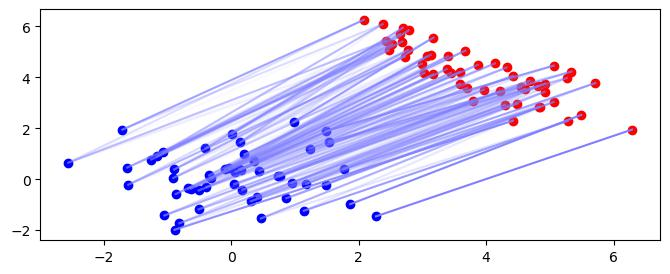
\includegraphics[width=0.5\textwidth]{chapter-2/images/0.001.jpg} & 
        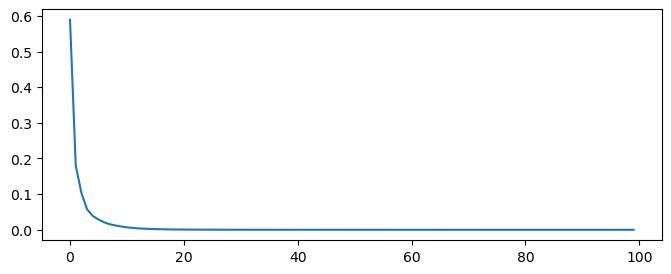
\includegraphics[width=0.5\textwidth]{chapter-2/images/err_0.001.jpg}\\
        \multicolumn{2}{c}{With $\epsilon=10^{-3}$.}\\[0.2cm]
        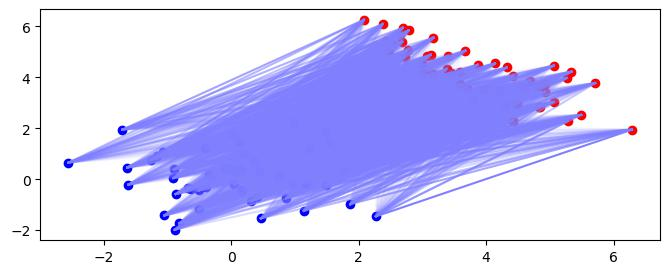
\includegraphics[width=0.5\textwidth]{chapter-2/images/0.1.jpg} & 
        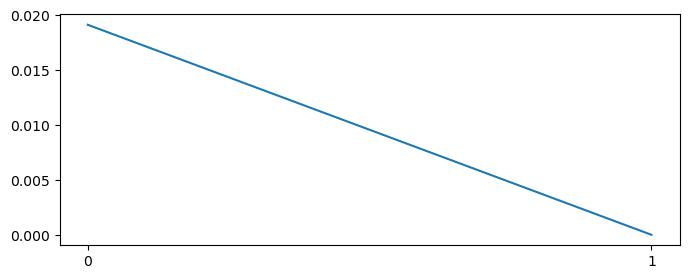
\includegraphics[width=0.5\textwidth]{chapter-2/images/err_0.1.jpg}\\
        \multicolumn{2}{c}{With $\epsilon=10^{-1}$.}\\
    \end{tabular}
    \caption[Illustration of the trade-off of the level of the sparsity of the OT plan and the numerical stability of the Sinkhorn algorithm for solving the entropy-regularized OT formulation.]{The OT plan (left) and the Convergence plot (right) are shown with different coefficients of entropic regularization ($\epsilon$). The non-zero values in the OT plan are shown as edges between the two sets of points (shown in red and blue). The color intensity of an edge represents the value corresponding to the two connecting points. Using $\epsilon=10^{-3}$ results in a sparser transport plan, but the Sinkhorn solver fails to converge even after 100 iterations. With $\epsilon=10^{-1}$, the convergence happens in just 1 iteration, but it results in a dense OT plan.}\label{fig:entr-sparsity}
\end{figure}